\section{Prioritising Brainstorm Ideas}

Due to the inherent limitations of the project, some functionality has to be excluded. To help determine which functionality should be the focus points, an evaluation was made according to the Risk Vs Value model to help prioritise the ideas. 

The Risk Vs Value model works by having the individual members of the development team evaluate each different functionality individually and giving them a risk and a value. Each of the values and risks is represented by a number from 0 to 100, where 100 value means that the functionality on its own will complete the project, and 0 provides nothing to the project. A 100 risk is something that will take all our time, and 0 is done without committing any time. 

In this project, each of the members of the development team wrote their evacuation without talking to each other or knowing the evaluation of the other members. Afterwards, the team revealed their numbers and the highest and the lowest would each explain why they evaluated it the way they did. After the explanation, the members of the group had the opportunity to change their evaluation. Using this approach produced the graph \ref{fig:RiskValueGraph}.

\begin{figure}[!h]
    \centering
	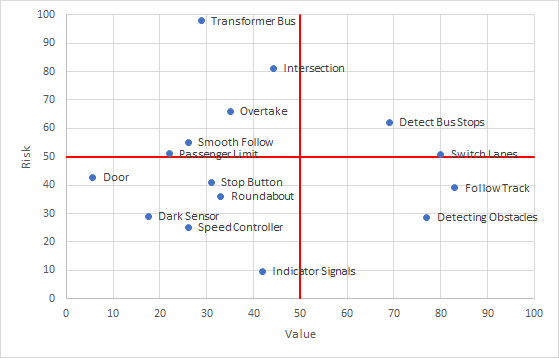
\includegraphics[width=0.9\textwidth]{Images/Graphs/RiskValue.png}
    \caption{Risk Value Graph}
    \label{fig:RiskValueGraph}
\end{figure}

According to the Risk Vs Value model, the development should start with the tasks with a high risk and value, then proceed with the tasks with low risk and high value, and lastly the tasks with low value and low risk. Where the tasks with high risk and low value should not be focused at all. 

According to the model, we should start detecting bus stops, and then prioritise the functionality according to a clockwise rotation. However there will never be any model that works as a silver bullet, and the relations and dependencies between the different functionality must be taken into account.  

\subsection{Priority Modifications}

In this section, we will give lower or higher priorities to some features, dependant on the relations between the different features.

All of the passenger functionality is completely reliant on the driving functionality. Because of this, everything concerning passengers was given low priority. The same reasoning is given to roundabouts, overtakes and intersections because these are also reliant on functional driving. Dark sensor is also given lower priority based on its low value.

Follow track is essential, which is why it has the highest value, to almost everything else, and has therefore been given higher priority.

